\section{Shared Directions Beyond Training Means}
\label{sec:mean-controls}
This section is the main evidence for C1 (main Sec.~\ref{M-sec:shared}). On held-out tasks and families of all 536 $\pi_{0.5}$ pairs, 16 shared directions retain 36.7--84.2\% of the response energy around the fitting-data mean, against 0.5--10.6\% for clean-feature and 1.3--1.9\% for random directions (Table~\ref{tab:mean-centered-controls}), for 1 to 32 directions alike (Sec.~\ref{sec:rank-sensitivity}). The result does not come from the mean: uncentered shared directions retain more raw energy than training-mean templates and their spans (Table~\ref{tab:mean-controls}). Of the raw energy the centered fit retains 16.26--75.00\%, lower in some cells for a reason given below. Section~\ref{sec:current-basis-readout} gives the 404-pair subset quoted in the main paper.

\subsection{Shared directions against mean and capacity controls}
\paragraph{Fits use fixed task/family splits.}
The analysis uses the first query, first generation step, ten ordered plan positions and 1,024 channels at each of L1, L9 and L18, fitted separately. Task components (tasks sharing a clean scene) are formed before folds are assigned; the original 60 joint task/family splits and 12 known-task, held-family splits are kept. Training weights are equal at each nested level (task component, family, setting, noise, position); test folds are joined before a family result, so each held-out component appears once. The families contribute 118/112/152/154 pairs and 34/32/40/39 task components; the full Light set includes 18 cases without a LIBERO-Plus difficulty level. Inputs, numbers of directions and fits do not use outcomes.

\paragraph{Every set of directions reconstructs the same residual about a training template.}
A global mean $\mu$ and ten position means $\mu_p$ use training data only, broadcast across positions or applied per position. Centered shared directions are fitted to $D-M$; centered clean-feature directions to clean features after subtracting their own training clean means; both, and the random directions, reconstruct the same residual $D-M$. Mean-only prediction has no test coefficients; the mean-direction and position-mean-span controls project the observed target (Sec.~\ref{sec:information-budget}), the latter with rank ten in every fold.

\paragraph{Scores are means of task ratios.}
For each held-out task component $t$, the score is one minus the reconstruction error $\mathrm{SSE}_t$ over the response energy, raw ($E_t$) or around the training template ($E_{M,t}$):
\begin{align}
 S_{\rm raw}&=\frac{1}{|\mathcal T|}\sum_{t\in\mathcal T}
 \left(1-\frac{\mathrm{SSE}_t}{E_t}\right),\\
 S_M&=\frac{1}{|\mathcal T|}\sum_{t\in\mathcal T}
 \left(1-\frac{\mathrm{SSE}_t}{E_{M,t}}\right).
\end{align}
Global and position templates give different residual energies. Zero denominators and too few directions are undefined. All primary comparisons have valid inputs and enough directions.

The tables report the primary comparisons with 16 directions on the original 72 training splits. Uncertainty uses 2,000 whole-task-component bootstrap draws shared across methods and numbers of directions, conditional on the fitted directions. All 95\% intervals are pointwise: paired difference intervals for the 16-direction contrasts, marginal intervals for the curves. Resampling preserves the dependence among family/layer comparisons, which share data and training support.

\begin{table*}[t]
\caption{\textbf{Uncentered shared directions retain more raw energy than training-mean templates and their spans.} Raw-energy scores $S_{\rm raw}$ (\%) under joint task/family holdout in the LIBERO-Plus recordings ($\pi_{0.5}$), by family (B/C/L/S: Background Textures, Camera Viewpoints, Light Conditions, Sensor Noise incl.\ blur and fog-like conditions) and layer. Shared (PCA16): 16 uncentered shared directions. Mean-only columns use no test response; the others project it, with 160, ten and 100 coefficients. Negative scores mean greater error than predicting zero. Point values; pointwise 95\% task-component intervals are in the text.}

\centering\small
\setlength{\tabcolsep}{7pt}
\begin{tabular}{lrrrrr}
\toprule
Family/layer & Shared (PCA16) & \shortstack{Global mean\\only} & \shortstack{Position mean\\only} & \shortstack{Global mean\\span} & \shortstack{Position-mean\\span}\\
\midrule
B / L1 & 55.63 & -47.41 & -48.76 & 11.68 & 29.46\\
B / L9 & 33.86 & -90.08 & -112.16 & 2.52 & 14.60\\
B / L18 & 32.51 & -94.23 & -112.92 & 3.56 & 13.55\\
C / L1 & 62.33 & -80.70 & -81.72 & 5.78 & 28.96\\
C / L9 & 64.66 & 0.92 & 1.64 & 6.42 & 22.36\\
C / L18 & 42.96 & 4.20 & 3.28 & 9.05 & 20.64\\
L / L1 & 49.27 & -272.46 & -277.68 & 3.06 & 30.43\\
L / L9 & 37.86 & -68.91 & -81.52 & 3.30 & 14.84\\
L / L18 & 32.37 & -47.67 & -56.72 & 3.53 & 13.63\\
S / L1 & 75.27 & 4.00 & 4.03 & 11.03 & 17.75\\
S / L9 & 47.16 & 4.45 & 4.80 & 12.07 & 24.82\\
S / L18 & 38.59 & 3.48 & 1.69 & 11.34 & 20.37\\
\bottomrule
\end{tabular}

\label{tab:mean-controls}
\end{table*}

\begin{table*}[t]
\caption{\textbf{Shared directions retain far more than clean-feature and random directions after centering; raw and around-mean shares.} Percent; same panel and holdouts. First two columns: raw shares $S_{\rm raw}$ of the 16 shared directions after global or position centering. Other columns: shares $S_M$ around the global or position training template for 16 shared (Response), clean-feature (Clean) and random (Random) directions, each with 160 coefficients from the test response. Means of task-component ratios; pointwise 95\% intervals are in the text. Both shares have the same error and different denominators: Light L1 retains 84.24\% around the position template and 45.48\% raw.}

\centering\small
\setlength{\tabcolsep}{5pt}
\begin{tabular}{lrrrrrrrr}
\toprule
 & \multicolumn{2}{c}{Raw share, shared directions} & \multicolumn{3}{c}{Share around global template} & \multicolumn{3}{c}{Share around position template}\\
Family/layer & Global & Position & Response & Clean & Random & Response & Clean & Random\\
\midrule
B / L1 & 54.87 & 54.63 & 65.19 & 2.53 & 1.33 & 65.28 & 2.53 & 1.33\\
B / L9 & 24.95 & 20.91 & 43.18 & 0.57 & 1.45 & 44.39 & 0.53 & 1.50\\
B / L18 & 24.65 & 16.26 & 38.55 & 9.65 & 1.60 & 39.30 & 8.12 & 1.63\\
C / L1 & 60.17 & 59.96 & 77.07 & 1.73 & 1.39 & 77.08 & 1.75 & 1.39\\
C / L9 & 64.92 & 64.82 & 64.07 & 0.53 & 1.65 & 63.70 & 0.50 & 1.63\\
C / L18 & 42.73 & 42.49 & 40.14 & 13.22 & 1.70 & 40.43 & 10.55 & 1.72\\
L / L1 & 46.42 & 45.48 & 84.28 & 1.91 & 1.85 & 84.24 & 1.90 & 1.84\\
L / L9 & 35.05 & 31.03 & 60.64 & 0.85 & 1.57 & 60.87 & 0.82 & 1.67\\
L / L18 & 29.16 & 24.19 & 50.85 & 7.72 & 1.92 & 50.55 & 6.90 & 1.90\\
S / L1 & 75.00 & 75.00 & 73.97 & 1.35 & 1.62 & 73.98 & 1.35 & 1.62\\
S / L9 & 46.81 & 46.96 & 43.73 & 0.61 & 1.39 & 43.46 & 0.61 & 1.39\\
S / L18 & 38.11 & 37.89 & 35.84 & 9.60 & 1.86 & 36.73 & 8.73 & 1.88\\
\bottomrule
\end{tabular}

\label{tab:mean-centered-controls}
\end{table*}

\subsection{What remains after centering}
\paragraph{The shared directions do more than the mean.}
The global and position mean-only predictors each have negative raw scores in seven of twelve cells (Table~\ref{tab:mean-controls}), yet the span of the position means reconstructs 13.5--30.4\% of the raw response energy. Uncentered shared directions reconstruct 32.4--75.3\%, with paired advantages of 18.2--57.5 percentage points over that span and positive pointwise intervals in all twelve cells. The span has rank ten, the shared directions sixteen; equal-size comparisons follow.

\paragraph{Centered shared directions keep a wide margin over clean-feature and random directions.}
With the training position template removed, the shared directions retain 36.7--84.2\% of the energy around the mean, against 0.5--10.6\% for centered clean-feature and 1.3--1.9\% for random directions (Table~\ref{tab:mean-centered-controls}). Around the global template they retain 35.8--84.3\%. Every paired pointwise interval favors the shared directions under both raw and around-mean scoring. Projection reduces or preserves error relative to mean-only prediction.

\paragraph{Raw and around-mean shares.}
With the position template, the shared directions retain 36.73--84.24\% of the energy around the mean and 16.26--75.00\% of the raw energy on this full 40-task panel (Table~\ref{tab:mean-centered-controls}); the main paper quotes the first on the 404-pair subset ($36.5$--$83.6\%$, Sec.~\ref{sec:current-basis-readout}) and the second from this table. The two differ only in the denominator. They are close where the fitting-data mean, learned without the test family, matches the held-out responses (Sensor Noise; Camera at L9 and L18). Where it does not, mean-only prediction has negative raw scores (Table~\ref{tab:mean-controls}), so the energy around the mean exceeds the raw energy and the raw share is lower (Background, Light, Camera at L1; largest for Light L1). Centering removes only the training template; an offset shared within the held-out family stays in the scored response.

\paragraph{The effect of position centering depends on the family and layer.}
On the common raw denominator, six cells have negative intervals for position-minus-global reconstruction, one has a small positive interval and five span zero. The positive cell is S/L9, $+0.151$ percentage points $[0.020,0.281]$. B/L9 and B/L18 have position-centered raw-share intervals that cross zero, 20.91\% $[-4.45,35.50]$ and 16.26\% $[-17.46,34.83]$: for Background at L9 and L18 the raw share of the centered fit is not distinguishable from zero.

Section~\ref{sec:current-basis-readout} reads commands from the position-centered directions, fitted with the same splits.

\subsection{Other numbers of directions}
\label{sec:rank-sensitivity}
The shared directions retain more than clean-feature and random directions for every number tested, $k\in\{1,4,8,16,32\}$ (Figs.~\ref{fig:supp-rank-joint} and~\ref{fig:supp-rank-known}), which supports C1's statement for other numbers of directions. It uses the 536-pair panel and all 72 training splits (60 joint task/family, 12 known-task, held-family). The 404 cases of Sec.~\ref{sec:current-basis-readout} give the main paper's paired reconstruction--readout comparison.

\paragraph{Matched targets and nested directions.}
For every $k$, shared, clean-feature and random directions reconstruct the same observed residual $D_p-\mu_p$ about the training position mean, with the same denominator. The shared and clean-feature curves use the leading $k$ directions of their training decompositions. Random directions are the first $k$ columns of one fixed 32-column orthonormal basis, whose first 16 also give Table~\ref{tab:mean-centered-controls}; the uncentered replication uses its own fixed random basis. Each uses $k$ coefficients of the observed response per position.

\paragraph{The ordering holds for all five numbers of directions.}
Shared directions retain more energy around the mean than clean-feature and random directions of equal number in every family/layer cell under both holdout settings. Under joint task/family holdout, the shared directions retain $7.0$--$66.0\%$ with one direction and $49.3$--$88.9\%$ with 32; with 32, clean-feature and random directions retain $1.0$--$15.0\%$ and $2.8$--$3.8\%$. Paired intervals against the controls are reported for the primary $k=16$, where every interval favors the shared directions in both settings.

\begin{figure*}[p]
\centering
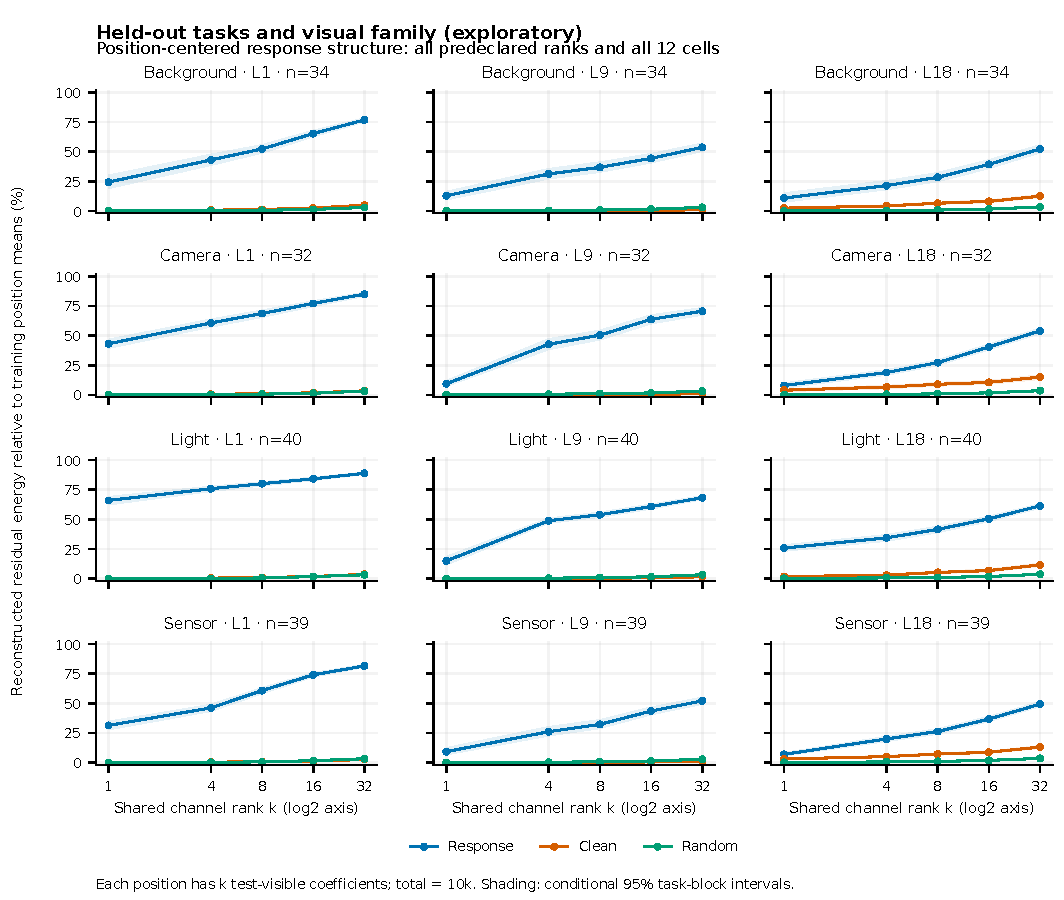
\includegraphics[width=\textwidth]{figures/r11_rank_joint.pdf}
\caption{\textbf{Shared directions retain more than clean-feature and random directions for every number of directions, under joint task/family holdout.} Shares of the energy around the training position means on the original 536-pair LIBERO-Plus panel, for $k=1,4,8,16,32$ directions. Twelve panels: four families by three layers; $34/32/40/39$ task components for Background/Camera/Light/Sensor Noise. Curves average task-component scores. Shading shows pointwise marginal 95\% intervals from 2,000 whole-component bootstrap draws conditional on the fits. Each set uses $k$ coefficients of the observed response per position, $10k$ in total.}
\label{fig:supp-rank-joint}
\end{figure*}

\begin{figure*}[p]
\centering
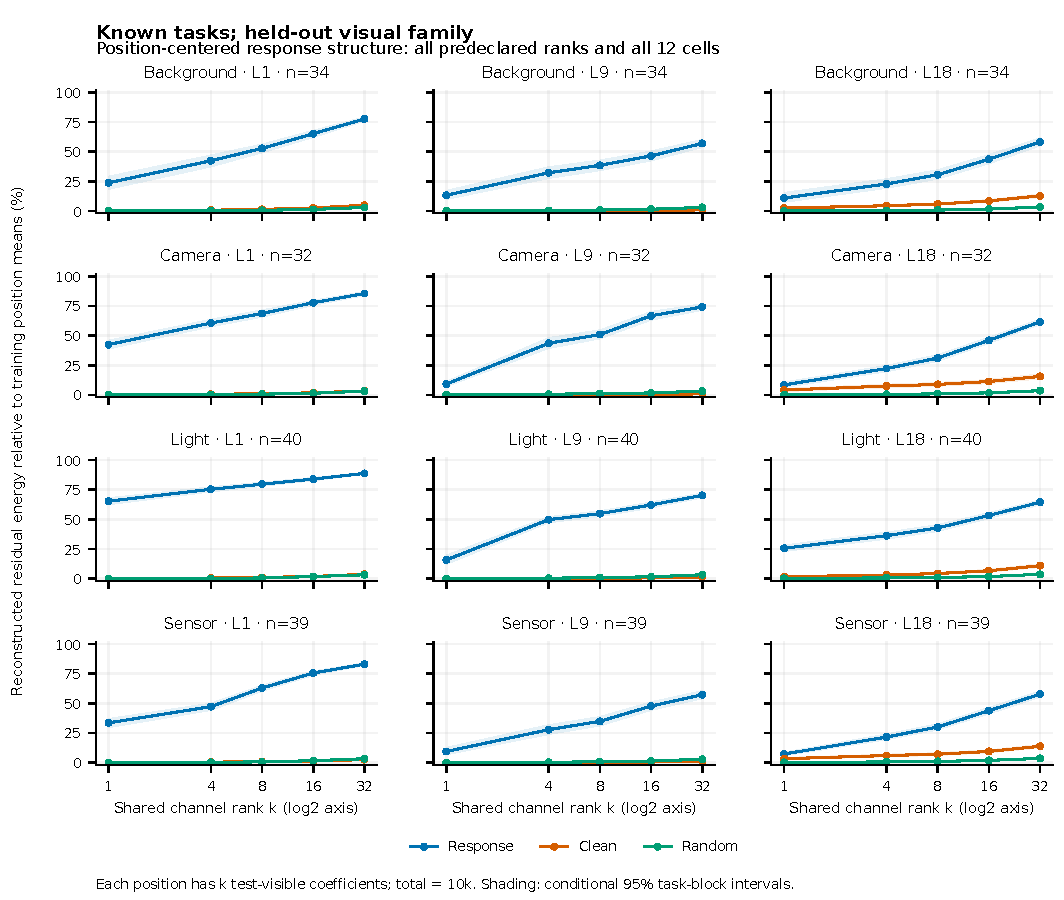
\includegraphics[width=\textwidth]{figures/r11_rank_known.pdf}
\caption{\textbf{The same ordering holds for known tasks and a held-out family.} The 536-pair panel under the twelve known-task, held-family splits; same target, denominator and $34/32/40/39$ task components as Fig.~\ref{fig:supp-rank-joint}. Shading shows pointwise marginal 95\% whole-task-component intervals conditional on the fits, using 2,000 shared draws. Each set uses $k$ coefficients of the observed response per position, $10k$ in total.}
\label{fig:supp-rank-known}
\end{figure*}
